% =====================================================================
%  Laborbericht 1 – Biosignalverarbeitung
%  Aufbau der Hardware & Datenakquise
%  Basierend auf der MCI-LaTeX-Vorlage (Drauschke/Teschl/Mehrle),
%  eigenständig kompilierbar (alle Definitionen in dieser Datei).
%
%  ROT markierte Stellen (\todo{...}) müssen noch ergänzt werden!
%  Max. 10 Seiten – vor der Abgabe Seitenzahl prüfen.
% =====================================================================

\documentclass[a4paper,oneside,10pt]{article}

\usepackage{ifthen}
\newboolean{english}
%\setboolean{english}{true}

% ---------------- Pakete & Layout (aus definitions.tex der Vorlage) ----
% Deutsche Silbentrennung: babel/ngerman bevorzugt, sonst Paket "german" der Vorlage
\IfFileExists{ngerman.ldf}{\usepackage[ngerman]{babel}}{%
  \IfFileExists{german.sty}{\usepackage{german}}{}}
\usepackage[T1]{fontenc}
\usepackage{lmodern}
\setlength{\emergencystretch}{2em}
\usepackage{graphicx}
\usepackage[tmargin=1in,bmargin=1in,lmargin=1.25in,rmargin=1.25in]{geometry}
\usepackage{titlesec}
\usepackage{xcolor}
\usepackage[overload]{textcase}
\definecolor{MSBlue}{rgb}{.204,.353,.541}
\definecolor{MSLightBlue}{rgb}{.31,.506,.741}
\titleformat{\section}[hang]{\rmfamily\bfseries\huge\color{MSBlue}}{\thesection}{1em}{\MakeLowercase}[]
\titleformat{\subsection}{\large\bfseries\sffamily\uppercase}{\thesubsection}{1em}{}
\titleformat{\subsubsection}{\sffamily\bfseries}{\thesubsubsection}{1em}{}
\def\litname{literatur}
\AtBeginDocument{%
  \renewcommand\contentsname{inhaltsverzeichnis.}%
  \renewcommand\listfigurename{abbildungsverzeichnis.}%
  \renewcommand\listtablename{tabellenverzeichnis.}%
  \renewcommand\refname{\litname.}%
  \renewcommand\figurename{Abbildung}%
  \renewcommand\tablename{Tabelle}}
\usepackage{fancyhdr}
\usepackage[small]{caption}
\usepackage{float}
\usepackage{amsmath,amssymb}
\usepackage{booktabs}
\usepackage{listings}
\setlength{\parindent}{0em}
\setlength{\parskip}{1.2ex plus0.5ex minus0.5ex}
\setlength{\captionmargin}{3em}

\lstset{basicstyle=\ttfamily\footnotesize,frame=single,columns=fullflexible,
        keywordstyle=\bfseries,language=C++,breaklines=true}

% ---------------- Platzhalter-Befehle --------------------------------
% \todo{Text}        -> roter Hinweis im Fließtext
% \platzhalter{Text} -> roter Rahmen anstelle einer noch fehlenden Abbildung
\newcommand{\todo}[1]{\textcolor{red}{\textbf{[TODO:} #1\textbf{]}}}
\newcommand{\platzhalter}[1]{%
  \fcolorbox{red}{white}{\parbox[c][4.2cm][c]{0.85\textwidth}{\centering
  \textcolor{red}{\textbf{PLATZHALTER -- Abbildung noch einfügen}}\\[1ex]
  \textcolor{red}{\small #1}}}}

% ---------------- Angaben Deckblatt ----------------------------------
\def\labtitle{Biosignalverarbeitung Laborbericht}
\def\labcode{BA-MGST-B-3-BB-BS-ILV}
\def\labname{Aufbau der Hardware \& Datenakquise}
\def\labnum{1}
\def\study{Medizin- Sport- und Gesundheitstechnik}
\def\term{3.}
\def\lecturer{Aitor Morillo}
\def\group{MGST-25}
\def\gruppennr{\textcolor{red}{X}} % TODO: Gruppennummer eintragen
\def\student{Matthias Zoller, Laurenz Keller, Matteo Harrasser}

\begin{document}

% =====================================================================
%  Deckblatt (aus deckblatt.tex)
% =====================================================================
\pagestyle{plain}
\thispagestyle{empty}
{\sffamily\bfseries
\vspace*{1cm}

\textcolor{MSBlue}{\rmfamily\bfseries\huge laborbericht.}

\vspace*{0.5cm}
\textbf{\labtitle{ }(\labcode)}

\labname

Labor \labnum{} -- Gruppe \gruppennr

\vspace*{10cm}
\textcolor{gray}{\study}

\textcolor{gray}{\term{ }Semester}

\textcolor{gray}{Lehrveranstaltungsleiter: \lecturer}

\textcolor{gray}{Jahrgang: \group}

\textcolor{gray}{Verfasser: \student}

\textcolor{gray}{\number\day.\,\number\month.\,\number\year}
\newpage}

\tableofcontents
\listoffigures
\listoftables
\newpage

\pagestyle{fancy}
\fancyhf{}
\fancyhead[L]{\small Laborbericht \labnum{} -- \labname}
\fancyhead[R]{\small Gruppe \gruppennr}
\fancyfoot[C]{\thepage}

% =====================================================================
\section{Einleitung}
% =====================================================================
Ziel des ersten Labors ist der Aufbau eines Messsystems zur Erfassung von
Beschleunigungsdaten sowie deren Verarbeitung in Python. Dazu wird ein
3-Achsen-Beschleunigungssensor über I\textsuperscript{2}C an einen
Mikrocontroller angebunden, die Daten über die serielle Schnittstelle an
einen PC übertragen und anschließend eingelesen, gefiltert und dargestellt.
Untersucht werden insbesondere die Auswirkung der Sensorkonfiguration
(Messbereich und Datenrate) auf die Qualität der Messdaten, die tatsächlich
erreichte Abtastfrequenz sowie der Unterschied zwischen stationärem
(USB) und mobilem (DataLogger, Batterie) Messsystem.

Der zugehörige Python-Code (\texttt{MainCode1.ipynb}) bearbeitet die
Aufgaben 4\,(a), 5, 6\,(a), 7, 8, 9 und 10 und ist zusammen mit allen
Datensätzen und dem modifizierten Arduino-Code der Abgabe beigelegt.

% =====================================================================
\section{Aufbau des Messsystems (Aufgabe 1)}
% =====================================================================
Abbildung~\ref{fig:messsystem} zeigt das stationäre Messsystem mit allen
Komponenten, Bussen und Signalpfaden.

\todo{Sensortyp prüfen! Im Blockschaltbild steht \emph{BMA400}, der
vorgegebene Code \texttt{Lab1Code1} verwendet aber die Bibliothek
\texttt{SparkFun\_MMA8452Q} (Sensor MMA8452Q, Default \texttt{ODR\_1}
= 1{,}56\,Hz statt 100\,Hz). Abbildung und Text an den tatsächlich verwendeten
Sensor anpassen. Die Aufgaben 3 und 5 unten sind für den MMA8452Q geschrieben.
Zusätzlich fehlt im Bild die Taktfrequenz des ATmega328P (16\,MHz).}

\begin{figure}[H]
    \centering
    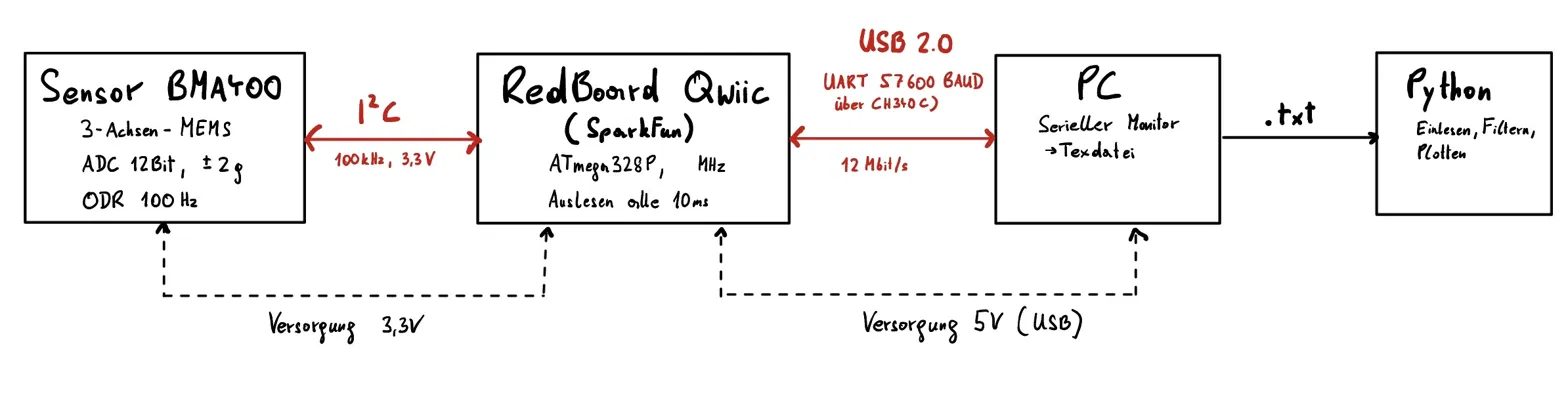
\includegraphics[width=\textwidth]{blockschaltbild.png}
    \caption{Blockschaltbild des stationären Messsystems mit Komponenten, Bussen und Signalpfaden.}
    \label{fig:messsystem}
\end{figure}

\subsection*{Komponenten}
\begin{description}
    \item[Beschleunigungssensor:] Digitaler 3-Achsen-MEMS-Beschleunigungssensor, der die
    Beschleunigung intern mit 12~Bit digitalisiert (Messbereich einstellbar,
    Standard $\pm 2\,g$). Die Werte werden mit der eingestellten Datenrate (ODR)
    in den Datenregistern bereitgestellt.
    \item[SparkFun RedBoard Qwiic:] Arduino-Uno-kompatibles Board mit dem
    Mikrocontroller ATmega328P (16~MHz), der den Sensor konfiguriert, die Rohdaten
    ausliest und jeden Messwert mit einem Zeitstempel (\texttt{millis()}) versieht.
    Ein USB-Seriell-Wandler (CH340C) leitet die Daten an den PC weiter.
    \item[PC (Serieller Monitor):] Der serielle Monitor der Arduino IDE empfängt die
    Messwerte zeilenweise als Text (\texttt{X Y Z Zeit}) und zeigt sie an. Die Daten
    werden anschließend per Copy \& Paste in einer Textdatei gespeichert.
    \item[Python:] Die Textdatei wird mit \texttt{pandas} eingelesen, mit
    \texttt{SciPy} gefiltert und mit \texttt{matplotlib} dargestellt und ausgewertet.
\end{description}

\subsection*{Busse und Signalpfade}
\begin{description}
    \item[I\textsuperscript{2}C (100~kHz, 3{,}3~V):] Serieller Zweidraht-Bus (SDA/SCL), über
    den das RedBoard den Sensor konfiguriert und die Messwerte ausliest.
    \item[USB 2.0 Full Speed (12~Mbit/s):] Überträgt die Messwerte vom RedBoard zum PC;
    die eigentliche Datenrate ist durch die UART-Verbindung zum CH340C auf
    57\,600~Baud begrenzt.
    \item[Datenpfad PC $\rightarrow$ Python:] Die Messdaten werden als Textdatei
    (\texttt{.txt}) an Python übergeben.
    \item[Spannungsversorgung:] Das RedBoard wird über USB mit 5~V versorgt und
    versorgt den Sensor über einen Spannungsregler mit 3{,}3~V.
\end{description}

% =====================================================================
\section{Vorausgehende Arbeiten und Berechnungen}
% =====================================================================

\subsection{Umrechnung eines ADC-Wertes in eine Temperatur (Aufgabe 2)}

Gegeben sind ein Temperatursensor mit Ausgangsspannung $U = 0 \ldots 3{,}3$\,V
für $\vartheta = 0 \ldots 40\,^\circ$C (linear) und ein Mikrocontroller-ADC mit
$n = 10$\,Bit und Referenzspannung $U_\mathrm{ref} = 5$\,V. Der ADC liefert
den Wert $D = 520$.

\textbf{Schritt 1 -- ADC-Wert in Spannung:} Mit $2^{10}-1 = 1023$ als
größtem Digitalwert gilt
\begin{equation}
  U = \frac{D}{2^{n}-1}\cdot U_\mathrm{ref} = \frac{520}{1023}\cdot 5\,\mathrm{V} \approx 2{,}542\,\mathrm{V}.
\end{equation}

\textbf{Schritt 2 -- Spannung in Temperatur:} Die Sensorkennlinie hat die
Empfindlichkeit $\frac{40\,^\circ\mathrm{C}}{3{,}3\,\mathrm{V}} \approx 12{,}12\,^\circ\mathrm{C/V}$:
\begin{equation}
  \vartheta = \frac{U}{3{,}3\,\mathrm{V}}\cdot 40\,^\circ\mathrm{C}
            = \frac{2{,}542\,\mathrm{V}}{3{,}3\,\mathrm{V}}\cdot 40\,^\circ\mathrm{C}
            \approx \mathbf{30{,}8\,^\circ C}.
\end{equation}

Rechnet man mit $2^{10} = 1024$ Stufen, ergibt sich $\vartheta \approx 30{,}78\,^\circ$C;
der Unterschied ist vernachlässigbar. Da der Sensor maximal 3{,}3\,V ausgibt, werden
nur $\frac{3{,}3}{5}\cdot 1023 \approx 675$ der 1024 Stufen genutzt; die effektive
Auflösung beträgt daher $\frac{40\,^\circ\mathrm{C}}{675} \approx 0{,}06\,^\circ$C pro Stufe.
\todo{Optional: kurzer Satz, warum 30{,}8\,°C unter der Körperkerntemperatur liegt (z.\,B. Hauttemperatur).}

\subsection{Achsenzuordnung und Umrechnung in physikalische Größen (Aufgabe 3)}

\textbf{Achsenzuordnung:} Der Arduino-Code gibt pro Zeile die Werte in der
Reihenfolge \texttt{getX()}, \texttt{getY()}, \texttt{getZ()} und anschließend
den Zeitstempel aus. Die erste Spalte entspricht somit der $x$-Achse, die
zweite der $y$-Achse und die dritte der $z$-Achse des auf der Platine
aufgedruckten Koordinatensystems.

\textbf{Test:} Im Ruhezustand misst der Sensor nur die Erdbeschleunigung.
Legt man den Sensor flach auf den Tisch (z-Achse nach oben), muss die dritte
Spalte ca.\ $+1\,g$ und die anderen beiden ca.\ $0\,g$ anzeigen. Kippt man den
Sensor nacheinander so, dass die $x$- bzw.\ $y$-Achse nach oben zeigt, muss
jeweils die entsprechende Spalte auf $+1\,g$ springen (nach unten: $-1\,g$).
\todo{Eigene Beobachtung beim Test kurz beschreiben (welche Spalte hat reagiert).}

\textbf{Einheit:} \texttt{getX()} usw.\ liefern den \emph{Rohwert} des 12-Bit-Datenregisters
als vorzeichenbehaftete ganze Zahl (Zweierkomplement, $-2048 \ldots +2047$) in
Digits (LSB), also noch keine physikalische Größe.

\textbf{Umrechnung:} Laut Datenblatt \cite{mma8452q} beträgt die Empfindlichkeit
$S = 1024$\,LSB/$g$ (Messbereich $\pm 2\,g$), $512$\,LSB/$g$ ($\pm 4\,g$) bzw.\
$256$\,LSB/$g$ ($\pm 8\,g$) \todo{Seite/Tabelle im Datenblatt eintragen}.
Damit gilt
\begin{equation}
  a\,[\mathrm{m/s^2}] = \frac{D_\mathrm{roh}}{S}\cdot g_0, \qquad g_0 = 9{,}81\,\mathrm{m/s^2}.
  \label{eq:umrechnung}
\end{equation}
Beispiel: Ein Rohwert von $1024$ bei $\pm 2\,g$ entspricht $1\,g = 9{,}81$\,m/s$^2$.

% =====================================================================
\section{Durchführung und Ergebnisse}
% =====================================================================

\subsection{Auf- und Abbewegung mit dem Originalcode (Aufgabe 4)}

Der Sensor wurde in der geschlossenen Hand gehalten und 10\,s lang einmal pro
Sekunde schnell auf und ab bewegt (ohne Rotation). Die Daten wurden mit dem
unveränderten Code \texttt{Lab1Code1} (\texttt{SCALE\_2G}, \texttt{ODR\_1})
aufgezeichnet und per Copy \& Paste in eine \texttt{.txt}-Datei übertragen.

\textbf{(a)} Abbildung~\ref{fig:a4} zeigt einen Ausschnitt von 4\,s der Messung.

\begin{figure}[H]
  \centering
  \platzhalter{Aufgabe 4(a): 4 s der Rohdaten (x, y, z) über der Zeit, Originalcode.
  Achsen: $t$/s und $a$/$g$; Kurven mit unterschiedlichem Linienstil + Legende.}
  \caption{Beschleunigung während der Auf- und Abbewegung mit dem Originalcode (Ausschnitt 4\,s).}
  \label{fig:a4}
\end{figure}

\textbf{(b) Plateaus der Peaks:} Die Peaks enden alle beim selben Wert, weil der
Sensor in die \emph{Sättigung} geht: Bei der Einstellung $\pm 2\,g$ kann das
12-Bit-Register maximal $+2047$ bzw.\ $-2048$ LSB ($\approx \pm 2\,g$) darstellen.
Beim schnellen Abbremsen und Umkehren der Hand treten jedoch größere
Beschleunigungen auf, sodass alle Werte darüber auf den Maximalwert
abgeschnitten werden (\emph{Clipping}). Lösen lässt sich das, indem man den
Messbereich im Register \texttt{XYZ\_DATA\_CFG} auf $\pm 4\,g$ oder $\pm 8\,g$
vergrößert (auf Kosten der Auflösung pro LSB).
\todo{Konkreten Plateau-Wert aus euren Daten angeben (z.\,B. ca.\ $\pm 2\,g$).}

\textbf{(c) Abweichung von der tatsächlichen Bewegung:} Neben dem Clipping ist
vor allem die Datenrate \texttt{ODR\_1} = 1{,}56\,Hz viel zu niedrig. Eine
schnelle Auf- und Abbewegung enthält Frequenzanteile deutlich über 1\,Hz; nach
dem Abtasttheorem müsste mit mehr als dem Doppelten der höchsten
Signalfrequenz abgetastet werden. Bei rund 1{,}5 Werten pro Sekunde wird pro
Bewegung höchstens ein bis zwei Punkte erfasst, kurze Spitzen fallen zwischen
die Abtastzeitpunkte und es kommt zu Aliasing. Zusätzlich misst der Sensor
immer auch die Erdbeschleunigung mit, und bereits kleine Verkippungen der Hand
verteilen diese auf mehrere Achsen.
\todo{Mit euren Beobachtungen aus Abb.~\ref{fig:a4} abgleichen.}

\subsection{Anpassung der Sensorkonfiguration (Aufgabe 5)}

Laut Datenblatt des MMA8452Q \cite{mma8452q} sind zwei Register relevant
(Tab.~\ref{tab:register}):

\begin{table}[H]
\centering
\small
\caption{Relevante Register des MMA8452Q und mögliche Parameterwerte.}
\label{tab:register}
\begin{tabular}{lll}
\toprule
Register / Parameter & mögliche Werte & Datenblatt \\
\midrule
\texttt{CTRL\_REG1} (0x2A), Bits \texttt{DR[2:0]} &
  800, 400, 200, 100, 50, 12{,}5, 6{,}25, 1{,}56\,Hz & S.~\todo{?} \\
\texttt{XYZ\_DATA\_CFG} (0x0E), Bits \texttt{FS[1:0]} &
  $\pm 2\,g$, $\pm 4\,g$, $\pm 8\,g$ (11 = reserviert) & S.~\todo{?} \\
\bottomrule
\end{tabular}
\end{table}

In der SparkFun-Bibliothek entsprechen diese den Funktionen
\texttt{setDataRate()} (\texttt{ODR\_800} \ldots{} \texttt{ODR\_1}) und
\texttt{setScale()} (\texttt{SCALE\_2G}, \texttt{SCALE\_4G}, \texttt{SCALE\_8G}).
Der Code wurde wie folgt geändert:

\begin{lstlisting}
accel.setScale(SCALE_8G);      // vorher SCALE_2G -> kein Clipping mehr
accel.setDataRate(ODR_100);    // vorher ODR_1 (1,56 Hz)
\end{lstlisting}
\todo{Prüfen, ob ihr genau diese Werte verwendet habt, sonst anpassen.}

\textbf{Begründung:} Menschliche Handbewegungen liegen im Wesentlichen unter
ca.\ 10--20\,Hz, eine Abtastrate von 100\,Hz erfüllt damit das Abtasttheorem
mit ausreichender Reserve. Höhere Raten sind über die serielle Verbindung nicht
sinnvoll: Eine Zeile (\texttt{X\textbackslash tY\textbackslash tZ\textbackslash tZeit\textbackslash r\textbackslash n})
umfasst ca.\ 26 Zeichen $\approx 260$\,Bit; bei 57\,600\,Baud sind damit nur
ca.\ 220 Zeilen/s übertragbar, 400 oder 800\,Hz würden also Daten verlieren.
Der Messbereich $\pm 8\,g$ verhindert die Sättigung aus Aufgabe 4; die
Auflösung von $1/256\,g \approx 0{,}04$\,m/s$^2$ ist für Bewegungen ausreichend.

Abbildung~\ref{fig:a5} zeigt die wiederholte Messung.

\begin{figure}[H]
  \centering
  \platzhalter{Aufgabe 5: 4 s der Daten mit geändertem Code (gleiche Achsenskalierung wie Abb. 2,
  damit der Vergleich leicht fällt).}
  \caption{Beschleunigung während der Auf- und Abbewegung mit angepasstem Messbereich und Datenrate (Ausschnitt 4\,s).}
  \label{fig:a5}
\end{figure}

\textbf{Vergleich:} \todo{Gemeinsamkeiten/Unterschiede zu Abb.~\ref{fig:a4} beschreiben, z.\,B.:}
Gemeinsam ist beiden Messungen die periodische Struktur mit etwa einer Bewegung
pro Sekunde sowie der Gleichanteil von ca.\ $1\,g$ in der vertikalen Achse
(Erdbeschleunigung). Im Unterschied zu Abb.~\ref{fig:a4} sind die Peaks nun
nicht mehr abgeschnitten, sondern zeigen die tatsächlichen Maximalwerte von
\todo{?}\,$g$, und der Signalverlauf ist durch die rund 64-fach höhere Datenrate
glatt und zeitlich fein aufgelöst. Dafür ist das Rauschen sichtbar, weil nun auch
kleine, schnelle Schwankungen erfasst werden.

\subsection{Zeitstempel und statische Messung in sechs Orientierungen (Aufgabe 6)}

Jede Messung wird direkt auf dem Mikrocontroller mit einem Zeitstempel versehen
(\texttt{millis()} \todo{bzw.\ \texttt{micros()} -- verwendete Funktion angeben}),
nicht über die Zeitstempel des seriellen Monitors. Aus den Zeitdifferenzen
$\Delta t_i = t_{i+1}-t_i$ werden in Python die mittlere Abtastfrequenz und
deren Streuung berechnet (siehe Abschnitt~\ref{sec:fs}).

Der Sensor wurde nacheinander in alle sechs Orientierungen gebracht
($\pm x$, $\pm y$, $\pm z$ jeweils nach oben) und jeweils 10\,s ruhig gehalten.

\textbf{(a)} Abbildung~\ref{fig:a6} zeigt die gesamte Messung.

\begin{figure}[H]
  \centering
  \platzhalter{Aufgabe 6(a): gesamte Messung der 6 Orientierungen (ca. 60 s), x/y/z über $t$/s,
  Werte in $g$; Abschnitte ggf. beschriften (+x oben, $-$x oben, ...).}
  \caption{Statische Messung in allen sechs Orientierungen des Sensors (je 10\,s).}
  \label{fig:a6}
\end{figure}

\textbf{(b) Plausibilität:} In Ruhe misst der Sensor nur die Erdbeschleunigung.
Zeigt eine Achse nach oben, sollte sie ca.\ $+1\,g$, nach unten ca.\ $-1\,g$ und
die beiden anderen Achsen ca.\ $0\,g$ anzeigen. (Ein Beschleunigungssensor
misst die Reaktionskraft der Unterlage, daher zeigt die nach oben gerichtete
Achse $+1\,g$.) \todo{Gemessene Mittelwerte je Orientierung angeben, z.\,B.
als kleine Tabelle, und Abweichungen von $\pm 1\,g$ diskutieren (Offset,
Verkippung von Hand, Empfindlichkeitstoleranz laut Datenblatt).}

\subsection{Filterung der Daten (Aufgabe 7)}

Die Daten aus Aufgabe~6 wurden mit einem digitalen Butterworth-Tiefpass
4.~Ordnung mit der Grenzfrequenz $f_g = $ \todo{?}\,Hz gefiltert. Damit das
Signal zeitlich nicht verschoben wird, wurde die Funktion \texttt{filtfilt()}
aus \texttt{scipy.signal} verwendet: Der Filter wird einmal vorwärts und einmal
rückwärts angewandt, wodurch die Phasenverschiebung aufgehoben wird
(Nullphasenfilter). Abbildung~\ref{fig:a7} vergleicht gefilterte und
ungefilterte Daten.

\begin{figure}[H]
  \centering
  \platzhalter{Aufgabe 7: ungefilterte (z.\,B. dünn, grau) vs. gefilterte Daten (durchgezogen) einer Achse
  bzw. aller Achsen; Ausschnitt so wählen, dass der Effekt gut sichtbar ist.}
  \caption{Vergleich der ungefilterten und mit einem Butterworth-Tiefpass gefilterten Beschleunigungsdaten.}
  \label{fig:a7}
\end{figure}

\textbf{Effekt und Begründung:} \todo{1--2 Sätze an eure Ergebnisse anpassen:}
Der Tiefpass entfernt das hochfrequente Sensor- und Quantisierungsrauschen,
sodass die Plateaus der einzelnen Orientierungen als glatte Werte bei ca.\
$\pm 1\,g$ bzw.\ $0\,g$ erscheinen, während die Übergänge zwischen den
Orientierungen erhalten bleiben. Ein Tiefpass wurde gewählt, weil die
interessierende Information (Lage bzw.\ langsame Bewegung) im niedrigen
Frequenzbereich liegt und das Rauschen breitbandig ist.

\subsection{Bestimmung der Abtastfrequenz (Aufgabe 8)}
\label{sec:fs}

Aus den Zeitstempeln der gesammelten Daten wurde die Abtastfrequenz berechnet:
\begin{equation}
  \bar f_s = \frac{1}{\overline{\Delta t}}, \qquad
  \overline{\Delta t} = \frac{1}{N-1}\sum_{i=1}^{N-1}(t_{i+1}-t_i), \qquad
  \sigma_{\Delta t} = \sqrt{\frac{1}{N-2}\sum_{i=1}^{N-1}\left(\Delta t_i-\overline{\Delta t}\right)^2}.
\end{equation}
Die Streuung der Frequenz wurde \todo{direkt aus $f_i = 1/\Delta t_i$ bzw.\ über
Fehlerfortpflanzung $\sigma_f \approx \sigma_{\Delta t}/\overline{\Delta t}^{\,2}$ -- Methode angeben}
bestimmt. Abbildung~\ref{fig:a8} zeigt die Verteilung der Abtastintervalle,
Tab.~\ref{tab:fs} die Ergebnisse.

\begin{figure}[H]
  \centering
  \platzhalter{Aufgabe 8: Histogramm der Abtastintervalle $\Delta t$/ms (oder $\Delta t$ über Sample-Index),
  Mittelwert als vertikale Linie einzeichnen.}
  \caption{Verteilung der Abtastintervalle des stationären Messsystems.}
  \label{fig:a8}
\end{figure}

\begin{table}[H]
\centering
\small
\caption{Abtastfrequenz des stationären (USB) und des mobilen (DataLogger) Messsystems.}
\label{tab:fs}
\begin{tabular}{lccc}
\toprule
Messsystem & $\overline{\Delta t}$ / ms & $\bar f_s$ / Hz & Standardabweichung $\sigma_f$ / Hz \\
\midrule
stationär (USB, Aufgabe 8)       & \todo{?} & \todo{?} & \todo{?} \\
mobil (DataLogger, Aufgabe 9)    & \todo{?} & \todo{?} & \todo{?} \\
\bottomrule
\end{tabular}
\end{table}

\todo{1--2 Sätze Interpretation: Stimmt $\bar f_s$ mit der eingestellten ODR (100\,Hz) überein?
Bei \texttt{millis()} ist die Auflösung nur 1\,ms, daher springen $\Delta t$ z.\,B. zwischen 9, 10 und 11\,ms.}

\subsection{Mobiles Messsystem (Aufgabe 9)}

Für diese Messung wurde das mobile Messsystem mit DataLogger und Batterie
verwendet. Mit dem Code \texttt{Lab1Code2} wurden ca.\ 10\,s aufgezeichnet und
die Abtastfrequenz analog zu Abschnitt~\ref{sec:fs} bestimmt
(Tab.~\ref{tab:fs}). \todo{Kurz beschreiben: welcher DataLogger, wie die Daten
gespeichert wurden (SD-Karte), Ergebnisse eintragen.}

\textbf{Diskussion:} \todo{An eure Messwerte anpassen, z.\,B.:}
Die mittlere Abtastfrequenz des mobilen Systems unterscheidet sich vom
stationären Wert und streut stärker. Ursache ist, dass der Mikrocontroller
die Daten nicht mehr nur seriell ausgibt, sondern an den DataLogger übergibt,
der sie auf eine SD-Karte schreibt. Das Schreiben erfolgt blockweise und
benötigt unregelmäßig mehrere Millisekunden, in denen keine neuen Werte
gelesen werden. Zudem unterscheiden sich der verwendete Code
(\texttt{Lab1Code2}, z.\,B.\ andere Datenrate oder Ausgabeformat), die
Übertragungsgeschwindigkeit zum Logger und die Taktquelle. Die eingestellte
Sensordatenrate stellt daher nur eine Obergrenze dar; die tatsächliche
Abtastfrequenz wird von der langsamsten Stelle der Signalkette bestimmt.

% =====================================================================
\section{Zusammenfassung}
% =====================================================================
\todo{3--5 Sätze Fazit, z.\,B.:} Das Messsystem aus Sensor, RedBoard und PC
wurde aufgebaut und in Betrieb genommen. Mit der Standardkonfiguration
($\pm 2\,g$, 1{,}56\,Hz) bildeten die Daten die Bewegung aufgrund von Sättigung
und zu geringer Abtastrate nicht korrekt ab. Durch die Anpassung von Messbereich
und Datenrate im Sensorregister konnte die Bewegung korrekt erfasst werden. Die
statische Messung bestätigte die Erdbeschleunigung von ca.\ $1\,g$ in jeder
Orientierung. Die tatsächlich erreichte Abtastfrequenz betrug \todo{?}\,Hz
(stationär) bzw.\ \todo{?}\,Hz (mobil).

% =====================================================================
% Literatur (IEEE-Stil, ohne BibTeX)
% =====================================================================
\begin{thebibliography}{9}
\bibitem{mma8452q}
NXP Semiconductors, ``MMA8452Q, 3-axis, 12-bit/8-bit digital accelerometer,'' Datenblatt,
Rev.~\todo{?}. \todo{Version/Link des verwendeten Datenblatts eintragen.}

\bibitem{redboard}
SparkFun Electronics, ``SparkFun RedBoard Qwiic -- Hookup Guide,'' online,
\todo{URL und Abrufdatum}.

\bibitem{scipy}
P.~Virtanen \emph{et al.}, ``SciPy 1.0: Fundamental algorithms for scientific computing in Python,''
\emph{Nature Methods}, vol.~17, pp.~261--272, 2020.

\bibitem{skript}
\todo{Vorlesungsunterlagen Biosignalverarbeitung (A.~Morillo), MCI, 2026 -- falls zitiert.}
\end{thebibliography}

% =====================================================================
\appendix
\section{Anhang: Abgegebene Dateien (Aufgabe 10)}
% =====================================================================
Die Abgabe \texttt{Lab1\_Gruppe\_\gruppennr.zip} enthält:
\begin{itemize}
  \item \texttt{Bericht\_1\_Gruppe\_\gruppennr.pdf} -- dieser Bericht,
  \item \texttt{Lab1Code1.ino} -- modifizierter Arduino-Code (Aufgabe 5),
  \item \texttt{MainCode1.ipynb} -- Python-Auswertung (Aufgaben 4a, 5, 6a, 7, 8, 9), erzeugt alle Abbildungen dieses Berichts,
  \item alle Datensätze (\texttt{.txt}), die für \texttt{MainCode1.ipynb} benötigt werden,
  \item ggf.\ selbstgeschriebene Python-Module. \todo{Liste an tatsächliche Dateinamen anpassen.}
\end{itemize}

\end{document}
